\documentclass{scrartcl}
        \usepackage{xcolor, tikz}
        \usepackage{pgfplots}
        \pgfplotsset{compat=newest}
        \pagestyle{empty}
        \definecolor{pdg2112}{RGB}{228,26,28}
\definecolor{pdg2212}{RGB}{55,126,184}
\definecolor{pdg1000010020}{RGB}{153,153,153}
\definecolor{pdg1000020040}{RGB}{166,86,40}
\definecolor{pdg11}{RGB}{152,78,163}
\definecolor{pdg1000010030}{RGB}{153,153,153}
\definecolor{pdg22}{RGB}{77,175,74}
\definecolor{pdg1000060120}{RGB}{153,153,153}
\definecolor{pdg1000020030}{RGB}{153,153,153}
\begin{document}
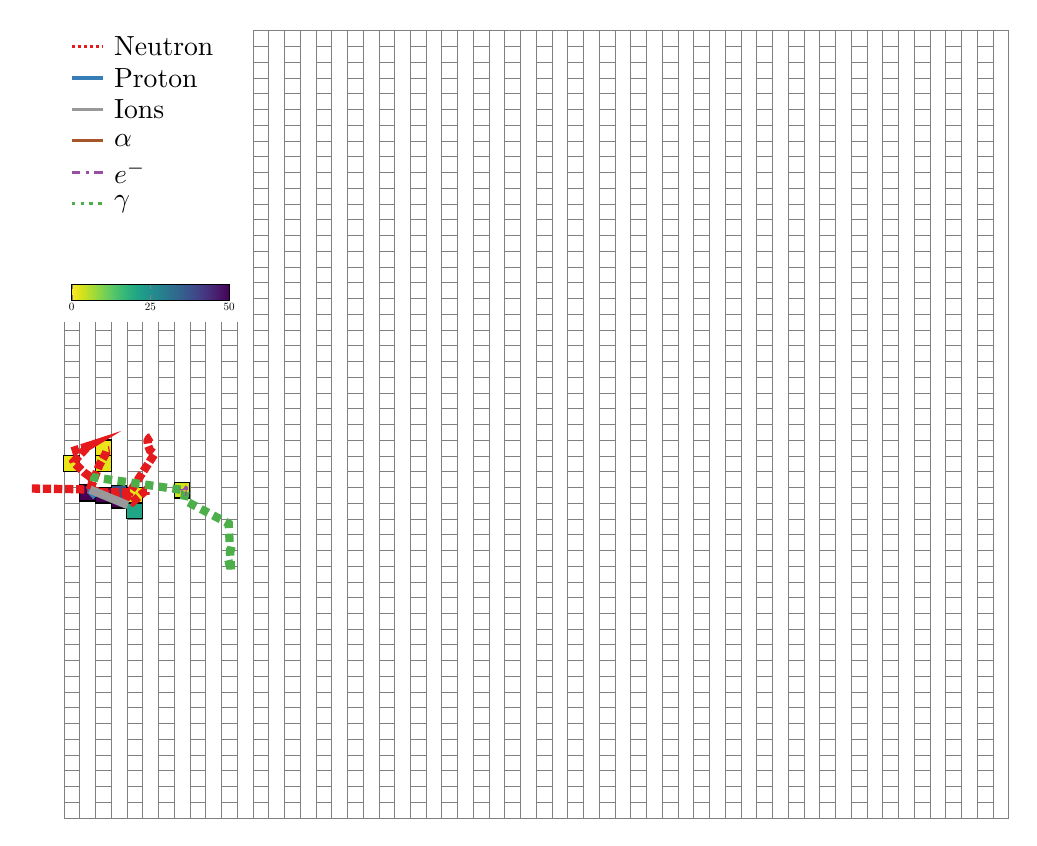
\begin{tikzpicture}[scale=0.4] %\columnwidth/252.0pt]
\draw[step=0.5,very thin,gray] (-0.001000,-12.499) grid (0.500000,3.25);
\draw[step=0.5,very thin,gray] (0.999000,-12.499) grid (1.500000,3.25);
\draw[step=0.5,very thin,gray] (1.999000,-12.499) grid (2.500000,3.25);
\draw[step=0.5,very thin,gray] (2.999000,-12.499) grid (3.500000,3.25);
\draw[step=0.5,very thin,gray] (3.999000,-12.499) grid (4.500000,3.25);
\draw[step=0.5,very thin,gray] (4.999000,-12.499) grid (5.500000,3.25);
\draw[step=0.5,very thin,gray] (5.999000,-12.499) grid (6.500000,12.499);
\draw[step=0.5,very thin,gray] (6.999000,-12.499) grid (7.500000,12.499);
\draw[step=0.5,very thin,gray] (7.999000,-12.499) grid (8.500000,12.499);
\draw[step=0.5,very thin,gray] (8.999000,-12.499) grid (9.500000,12.499);
\draw[step=0.5,very thin,gray] (9.999000,-12.499) grid (10.500000,12.499);
\draw[step=0.5,very thin,gray] (10.999000,-12.499) grid (11.500000,12.499);
\draw[step=0.5,very thin,gray] (11.999000,-12.499) grid (12.500000,12.499);
\draw[step=0.5,very thin,gray] (12.999000,-12.499) grid (13.500000,12.499);
\draw[step=0.5,very thin,gray] (13.999000,-12.499) grid (14.500000,12.499);
\draw[step=0.5,very thin,gray] (14.999000,-12.499) grid (15.500000,12.499);
\draw[step=0.5,very thin,gray] (15.999000,-12.499) grid (16.500000,12.499);
\draw[step=0.5,very thin,gray] (16.999000,-12.499) grid (17.500000,12.499);
\draw[step=0.5,very thin,gray] (17.999000,-12.499) grid (18.500000,12.499);
\draw[step=0.5,very thin,gray] (18.999000,-12.499) grid (19.500000,12.499);
\draw[step=0.5,very thin,gray] (19.999000,-12.499) grid (20.500000,12.499);
\draw[step=0.5,very thin,gray] (20.999000,-12.499) grid (21.500000,12.499);
\draw[step=0.5,very thin,gray] (21.999000,-12.499) grid (22.500000,12.499);
\draw[step=0.5,very thin,gray] (22.999000,-12.499) grid (23.500000,12.499);
\draw[step=0.5,very thin,gray] (23.999000,-12.499) grid (24.500000,12.499);
\draw[step=0.5,very thin,gray] (24.999000,-12.499) grid (25.500000,12.499);
\draw[step=0.5,very thin,gray] (25.999000,-12.499) grid (26.500000,12.499);
\draw[step=0.5,very thin,gray] (26.999000,-12.499) grid (27.500000,12.499);
\draw[step=0.5,very thin,gray] (27.999000,-12.499) grid (28.500000,12.499);
\draw[step=0.5,very thin,gray] (28.999000,-12.499) grid (29.500000,12.499);
\draw[very thin,gray] (0,-12.5) -- (30,-12.5) -- (30,12.5) -- (6,12.5);
\definecolor{tempcolor}{rgb}{0.916242,0.896091,0.100717}\draw[fill=tempcolor,fill opacity=1] (0.000000,-1.500000) rectangle (0.500000,-1.000000);
\definecolor{tempcolor}{rgb}{0.886271,0.892374,0.095374}\draw[fill=tempcolor,fill opacity=1] (0.500000,-2.461008) rectangle (1.000000,-1.961008);
\definecolor{tempcolor}{rgb}{0.267004,0.004874,0.329415}\draw[fill=tempcolor,fill opacity=1] (0.500000,-2.425836) rectangle (1.000000,-1.925836);
\definecolor{tempcolor}{rgb}{0.267004,0.004874,0.329415}\draw[fill=tempcolor,fill opacity=1] (1.000000,-2.500000) rectangle (1.500000,-2.000000);
\definecolor{tempcolor}{rgb}{0.886271,0.892374,0.095374}\draw[fill=tempcolor,fill opacity=1] (1.000000,-1.500000) rectangle (1.500000,-1.000000);
\definecolor{tempcolor}{rgb}{0.926106,0.897330,0.104071}\draw[fill=tempcolor,fill opacity=1] (1.000000,-1.000000) rectangle (1.500000,-0.500000);
\definecolor{tempcolor}{rgb}{0.267004,0.004874,0.329415}\draw[fill=tempcolor,fill opacity=1] (1.500000,-2.656167) rectangle (2.000000,-2.156167);
\definecolor{tempcolor}{rgb}{0.229739,0.322361,0.545706}\draw[fill=tempcolor,fill opacity=1] (1.500000,-2.437214) rectangle (2.000000,-1.937214);
\definecolor{tempcolor}{rgb}{0.130067,0.651384,0.521608}\draw[fill=tempcolor,fill opacity=1] (2.000000,-3.000000) rectangle (2.500000,-2.500000);
\definecolor{tempcolor}{rgb}{0.896320,0.893616,0.096335}\draw[fill=tempcolor,fill opacity=1] (2.000000,-2.500000) rectangle (2.500000,-2.000000);
\definecolor{tempcolor}{rgb}{0.824940,0.884720,0.106217}\draw[fill=tempcolor,fill opacity=1] (3.500000,-2.338902) rectangle (4.000000,-1.838902);
\draw[color=pdg2112, line width=3pt, densely dotted] (-1.015924663337728, -2.0400919386444825) -- (-0.01603154027288838, -2.0537838308501497) -- (0.0029999999999972713, -2.0540444365008073) -- (0.21685728662639575, -2.0569728603976634) -- (0.48999999999998634, -2.0640839328917067) -- (0.833614947296428, -2.073029698898357);
\draw[color=pdg1000020030, line width=3pt, solid] (0.833614947296428, -2.073029698898357);
\draw[color=pdg2212, line width=3pt, solid] (0.833614947296428, -2.073029698898357) -- (0.8790210772570617, -2.1229707003491796) -- (0.915236176920439, -2.162986164939552) -- (0.9435443253575613, -2.195417619550605) -- (0.9662092914996038, -2.220983227767074) -- (0.9841984321571999, -2.2416127876403764) -- (1.0029999999999972, -2.2634279499264744) -- (1.019366284172611, -2.281934595722979) -- (1.0270293675944686, -2.2900420601992626);
\draw[color=pdg2112, line width=3pt, densely dotted] (0.833614947296428, -2.073029698898357) -- (0.9899999999999863, -2.1178207209882776) -- (1.0029999999999972, -2.121544115757165) -- (1.1388751746588697, -2.160460801491537);
\draw[color=pdg1000020040, line width=3pt, solid] (1.1388751746588697, -2.160460801491537);
\draw[color=pdg1000010030, line width=3pt, solid] (1.1388751746588697, -2.160460801491537);
\draw[color=pdg1000020040, line width=3pt, solid] (1.1388751746588697, -2.160460801491537);
\draw[color=pdg2112, line width=3pt, densely dotted] (1.1388751746588697, -2.160460801491537) -- (1.490000000000009, -2.1582774010845522) -- (1.9899999999999864, -2.155168249795031) -- (2.100031671720262, -2.154484039566996) -- (2.192979308254871, -2.01) -- (2.490000000000009, -1.548291117683852) -- (2.5029999999999974, -1.5280830458662387) -- (2.8783099856480248, -0.9446760348006974) -- (2.7358303554962276, -0.8248332182528497) -- (2.7107610384478904, -0.7637423576116891) -- (2.70552251311949, -0.7509767118549177) -- (2.7010323485522805, -0.7400347297776847) -- (2.6972905447462834, -0.7309164113799909) -- (2.677178381650356, -0.6815055153725774) -- (2.6747454098765275, -0.662550594643584) -- (2.6582254302339834, -0.533845893693621) -- (2.6895662378175076, -0.46681663341576424) -- (2.7319925516340846, -0.41953999981738876) -- (2.750400267589066, -0.41433056038519417) -- (2.788632283496554, -0.3898949556751167);
\draw[color=pdg2212, line width=3pt, solid] (2.677178381650356, -0.6815055153725774);
\draw[color=pdg2212, line width=3pt, solid] (2.100031671720262, -2.154484039566996);
\draw[color=pdg2212, line width=3pt, solid] (1.1388751746588697, -2.160460801491537);
\draw[color=pdg2112, line width=3pt, densely dotted] (0.833614947296428, -2.073029698898357) -- (0.9342630354759194, -1.8052350695993795) -- (0.9390354195754981, -1.7925371748460937) -- (0.9431260345179908, -1.7816532650575632) -- (0.9465348803034204, -1.7725833402337874) -- (0.9899999999999863, -1.6569355835091266) -- (0.99699999999998, -1.6383106653512622) -- (1.0029999999999746, -1.6223464497873181) -- (1.0079999999999927, -1.6090429368173464) -- (1.0452243545900957, -1.5099999999999998) -- (1.1279565277622168, -1.2898742922348299) -- (1.2866078538372676, -1.0100000000000002) -- (1.32103349797826, -0.9492702662685237) -- (1.3590747049162246, -0.8400262972884767) -- (1.4575746952720692, -0.8235135667973636);
\draw[color=pdg2212, line width=3pt, solid] (1.4575746952720692, -0.8235135667973636);
\draw[color=pdg2212, line width=3pt, solid] (1.3590747049162246, -0.8400262972884767);
\draw[color=pdg2212, line width=3pt, solid] (1.1279565277622168, -1.2898742922348299);
\draw[color=pdg2212, line width=3pt, solid] (0.833614947296428, -2.073029698898357) -- (0.8148871099863527, -2.083016437057893) -- (0.7999683221082023, -2.091290491958394) -- (0.7881912641863664, -2.0981729713813158) -- (0.7786659813675897, -2.1036838554102286) -- (0.7710939007891284, -2.1082427372293666);
\draw[color=pdg1000010020, line width=3pt, solid] (0.833614947296428, -2.073029698898357) -- (0.8604160606379991, -2.0650743743552025) -- (0.8818435897162317, -2.0584322207274828) -- (0.898912216424651, -2.0532222974447394) -- (0.9125341374613753, -2.049135202890038) -- (0.9233060190375, -2.045748658293266);
\draw[color=pdg2112, line width=3pt, densely dotted] (0.833614947296428, -2.073029698898357) -- (0.9899999999999863, -2.109553349768412) -- (1.4899999999999864, -2.226328099780121) -- (1.9899999999999864, -2.3431028497918303) -- (2.02565367761531, -2.3514297483728823) -- (2.0535856622069333, -2.401342729333858) -- (2.1836873109711634, -2.468178220682481) -- (2.3630926242561143, -2.3127900103678063) -- (2.490000000000009, -2.2005726199264477) -- (2.5029999999999974, -2.1890774166950755) -- (2.6032633450505274, -2.100419914540149) -- (2.6060666482674604, -2.100582093437823) -- (2.6393291379447192, -2.1025064210942683) -- (2.592162869100025, -2.1152552685970223) -- (2.5913831619500343, -2.2373561583206083);
\draw[color=pdg2212, line width=3pt, solid] (2.1836873109711634, -2.468178220682481);
\draw[color=pdg2212, line width=3pt, solid] (2.0535856622069333, -2.401342729333858);
\draw[color=pdg2112, line width=3pt, densely dotted] (0.833614947296428, -2.073029698898357) -- (0.9181187872301735, -1.7834665016004994);
\draw[color=pdg1000020040, line width=3pt, solid] (0.9181187872301735, -1.7834665016004994);
\draw[color=pdg1000020040, line width=3pt, solid] (0.9181187872301735, -1.7834665016004994);
\draw[color=pdg1000020040, line width=3pt, solid] (0.9181187872301735, -1.7834665016004994);
\draw[color=pdg2112, line width=3pt, densely dotted] (0.9181187872301735, -1.7834665016004994) -- (0.8384311924348367, -1.6676418661716585);
\draw[color=pdg22, line width=3pt, dotted] (0.8384311924348367, -1.6676418661716585) -- (0.9899999999999863, -1.6892190398541238) -- (1.0029999999999972, -1.6910697059798134) -- (1.4899999999999864, -1.760398506226808) -- (1.5029999999999972, -1.7622491723524978) -- (1.7288033852243643, -1.7943943012833325) -- (1.9899999999999864, -1.8315779725994954) -- (2.0029999999999974, -1.8334286387251848) -- (2.4899999999999864, -1.9027574389721795) -- (2.5029999999999974, -1.9046081050978692) -- (2.769766401177594, -1.9425846852618354) -- (2.990000000000009, -1.973936905344868) -- (3.0029999999999974, -1.9757875714705544) -- (3.1028351719513694, -1.9899999999999998) -- (3.1168841674125587, -1.9920000000000002) -- (3.152006656065532, -1.9969999999999999) -- (3.1941536424491233, -2.003) -- (3.2292761311020968, -2.008) -- (3.243325126563286, -2.0100000000000002) -- (3.490000000000009, -2.0451163717175502) -- (3.5029999999999974, -2.0469670378432365) -- (3.8055891379012565, -2.0900433045752) -- (3.8131947428082187, -2.0959770521769534) -- (3.8654527175259092, -2.1367477253774454) -- (3.847457227505197, -2.2267134361180885) -- (3.84337970863844, -2.2470983704812744) -- (3.8398846924669443, -2.264571171364005) -- (3.836972178990686, -2.279131838766282) -- (3.8120817758871, -2.4035676170228046) -- (3.990000000000009, -2.4972101174355736) -- (4.490000000000032, -2.7603717493585282) -- (4.524627447002376, -2.778596980283463) -- (4.534207465963436, -2.78363916713075) -- (4.542190815097638, -2.787840989503489) -- (4.990000000000009, -3.0235333812814744) -- (5.234452380978451, -3.1521943562929415) -- (5.251782334869108, -3.4899999999999998) -- (5.277433111008395, -3.9900000000000007) -- (5.303083887147659, -4.49) -- (5.312671125707675, -4.676880087136092) -- (5.272542516948579, -4.51) -- (5.224801311163605, -4.3114619288397495) -- (5.294779995374029, -4.01) -- (5.361220683963552, -3.7237794406734985);
\draw[color=pdg11, line width=3pt, dashdotted] (3.8120817758871, -2.4035676170228046);
\draw[color=pdg11, line width=3pt, dashdotted] (3.8654527175259092, -2.1367477253774454) -- (3.8820167950895437, -2.1394482237583903) -- (3.897029170811834, -2.140075303002647);
\draw[color=pdg11, line width=3pt, dashdotted] (3.8055891379012565, -2.0900433045752) -- (3.8065401802557517, -2.0583820425773416) -- (3.788846230552008, -2.045934360991077);
\draw[color=pdg1000060120, line width=3pt, solid] (0.8384311924348367, -1.6676418661716585);
\draw[color=pdg2112, line width=3pt, densely dotted] (0.8384311924348367, -1.6676418661716585) -- (0.6349965411330458, -1.5217203628865952) -- (0.5100000000000137, -1.3989288985906019) -- (0.3211582889299052, -1.213418563566377) -- (0.3121875586453825, -1.1896094288685564) -- (0.47868290571464056, -1.0100000000000002) -- (0.48517180463732074, -1.0030000000000001) -- (0.49073371799959203, -0.9970000000000001) -- (0.4970000000000255, -0.9902401514454671) -- (0.5029999999999746, -0.9837675587143409) -- (0.5079999999999927, -0.9783737314383523) -- (0.5298739533008302, -0.9547768662489153) -- (0.7166966875531215, -0.7532389542930149) -- (0.7591842068728966, -0.707404886174062) -- (0.8006714155423651, -0.6820500648396481) -- (0.611588479245188, -0.7435957853644222) -- (0.5100000000000137, -0.7766624188460188) -- (0.2557769350938088, -0.8594109841585272);
\draw[color=pdg2212, line width=3pt, solid] (0.2557769350938088, -0.8594109841585272);
\draw[color=pdg2212, line width=3pt, solid] (0.3121875586453825, -1.1896094288685564);
\draw[color=pdg2212, line width=3pt, solid] (0.3211582889299052, -1.213418563566377);
\draw[color=pdg1000010020, line width=3pt, solid] (0.833614947296428, -2.073029698898357) -- (0.9503081831430791, -2.120742297232421) -- (0.9899999999999863, -2.1368106074288447) -- (1.219771559439596, -2.2318083268420734) -- (1.3896403147505225, -2.3012101562350322) -- (1.490000000000009, -2.344133238870252) -- (1.6228477988161103, -2.3981411616505612) -- (1.7116474776054929, -2.43336438102527) -- (1.7419838699633374, -2.445852750167873) -- (1.817241780564018, -2.4777006816776166) -- (1.8649629320860412, -2.4984217658823114) -- (1.9029446482994898, -2.5148763849143214) -- (1.9332607626980007, -2.527935782120568) -- (1.9574569395475465, -2.5382793695549637) -- (1.9761865865775008, -2.54619520743979) -- (1.990000000000009, -2.5515199848794134) -- (2.0029999999999974, -2.556608767514952) -- (2.0184825281181475, -2.5627716380015637) -- (2.02541170662123, -2.5652751906587357) -- (2.0310197599240154, -2.5673120681940604);
\draw[color=pdg1000060120, line width=3pt, solid] (0.21685728662639575, -2.0569728603976634);
\draw[color=pdg2112, very thick, densely dotted] (0.25,12) -- (1.25,12) node [right,black] {Neutron};
\draw[color=pdg2212, very thick, solid] (0.25,11) -- (1.25,11) node [right,black] {Proton};
\draw[color=pdg1000010020, very thick, solid] (0.25,10) -- (1.25,10) node [right,black] {Ions};
\draw[color=pdg1000020040, very thick, solid] (0.25,9) -- (1.25,9) node [right,black] {$\alpha$};
\draw[color=pdg11, very thick, dashdotted] (0.25,8) -- (1.25,8) node [right,black] {$e^-$};
\draw[color=pdg22, very thick, dotted] (0.25,7) -- (1.25,7) node [right,black] {$\gamma$};

        \begin{axis}[%
            at={(0.25cm,4.75cm)},
            hide axis,
            scale only axis,
            height=0pt,
            width=0pt,
            colormap={reverse viridis}{
                indices of colormap={
                \pgfplotscolormaplastindexof{viridis},...,0 of viridis}
            },
            colorbar horizontal,
            point meta min=0,
            point meta max=50,
            colorbar style={
                width=5cm,
                xtick={50, 25, 0},
            }]
        \end{axis}
        
        \end{tikzpicture}
        \end{document}
        